\chapter{Implementation}
\label{implementation}
In this chapter, we show an overview of all the implementation tools and procedures that we used to create KamehaMail. The implementation is separated into two major parts: the backend which communicates with the mailserver and the search engine, and the browser-based frontend that provides an interface to the end-user. These two parts communicate with each other using API calls.

\section{Backend}
 The implementation of the backend follows the usual style of deployment of PHP application. The software on the server is organized as follows:
\begin{itemize}
\item \emph{Apache HTTP server} is used to serve the static frontend files and the end-user's web browser, and provides the translation of the browser-originated HTTP API calls to the PHP application.
\item The application is run by \emph{PHP} with several additional modules (the complete list is shown in \autoref{userguide}).
\item The application communicates with \emph{Exim4} mail server using standard UNIX methods: \texttt{sendmail} for sending e-mail and pipe-based transport for receiving. Exim handles the communication with the e-mail infrastructure using standard internet protocols. It is also possible to integrate other mail servers.
\item \emph{ElasticSearch} is installed for searching and indexing the e-mails. The server communicates with it via REST API using \texttt{curl} requests.
\end{itemize}

\subsection{Data storage}
The data on the server are stored on two different places: the primary storage of the e-mails as files in user directories, and the secondary indexed storage in ElasticSearch.

The primary storage is organized as follows: in a specified directory 
the application stores the meta-information about users
(e.g. login details) and the users' mailboxes.

The mailbox section contains all the stored e-mails. Each e-mail is uniquely identified by its 64-character Sha-256 hash. The e-mails are separated into users' subdirectories, in which they are further separated into a subdirectory structure based on first few characters of the hash, to minimize the problems with large directories.

The meta-information section contains two SQLite databases, \texttt{usersdb} and \texttt{loginkeys}. \texttt{usersdb} is a list of all users and their corresponding passwords. \texttt{loginkeys} is a list of the currently logged users and their corresponding login API keys (further explained in \autoref{userapi}).

The directory hierarchy is displayed in \autoref{fig:folder-tree}.
 \begin{figure}
\centering
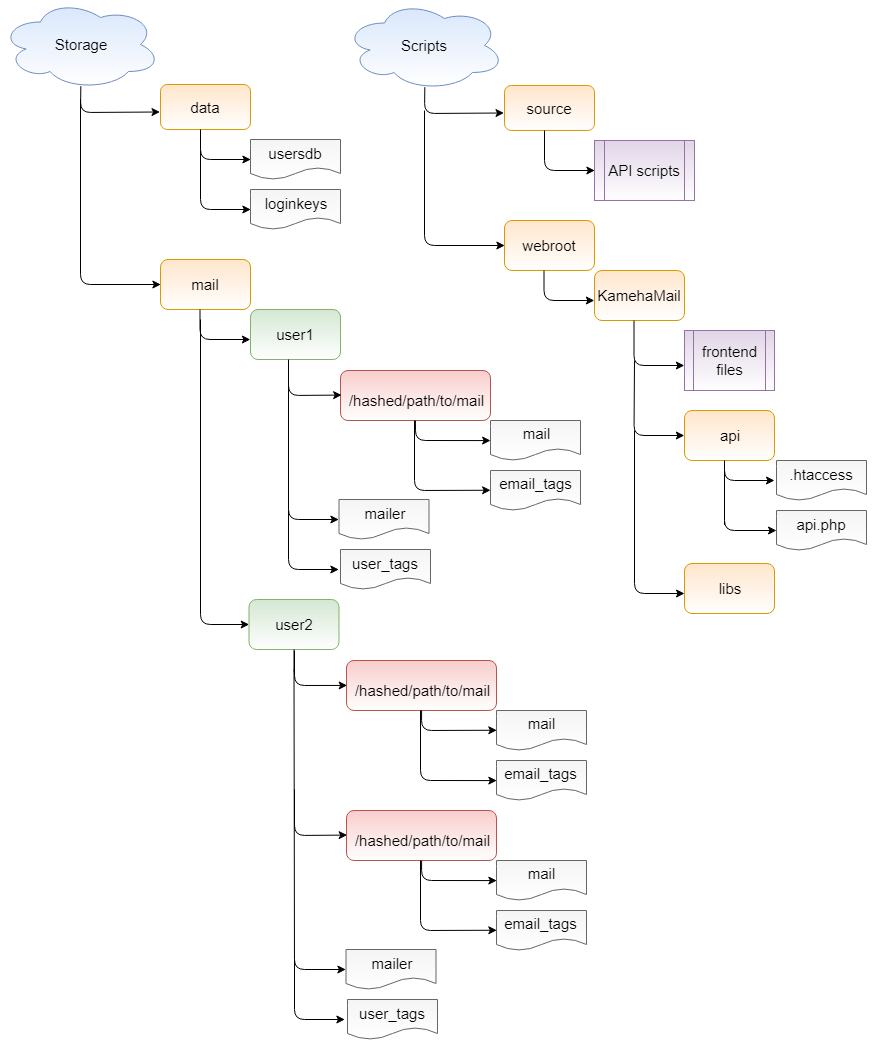
\includegraphics[width=\textwidth]{img/folder_tree.png}
\caption{A folder hierarchy on the server}
\label{fig:folder-tree}
\end{figure}

\subsection{API}
All of the server side scripting was done in PHP. To simplify the communication between the frontend and the backend, we created a set of API calls which run specific PHP scripts.

To provide REST-like API calls, htaccess is used. If an HTTP request is directed to the folder where the \texttt{.htaccess} is located, \texttt{htaccess} takes the request's URL and forwards it as a query string to a beforehand defined script. For example, upon calling URL
\begin{center}
\texttt{hruska.blesmrt.cf/KamehaMail/api/some-work}
\end{center}
htaccess takes a part of the url after its folder's name (i.e. \texttt{some-work}) and sends it to the \texttt{api.php} as a query string. \texttt{api.php} serves as a relay or a router. It loads all necessary source scripts and calls other PHP scripts accordingly to the received query string.

We provide an example of the processing of the user login API request:
\begin{enumerate}
\item  A HTTP POST request is sent from the frontend to the URL\\\texttt{api/client/login} with the data: \texttt{username} and \texttt{password}.
\item \texttt{.htaccess} in the api folder processes the url string and redirects\\\texttt{client/login} as a query string to the \texttt{api.php}.
\item \texttt{api.php} parses the query string, calls an external \texttt{login} function (defined by \texttt{login.php} in the source folder) with the username and password as parametres.
\item The login function checks the credentials and returns a JSON formatted response whether the login was successful or not, together with a new API key (which is simultaneously stored to the \texttt{loginkeys} database).
\item Then \texttt{api.php} forwards the response to the frontend.
\end{enumerate}

The source folder contains many of the PHP scripts for different uses. In the \autoref{fig:folder-tree}, they are denoted as \texttt{API scripts}. Depending on their purpose, they can be divided into three categories:

\subsubsection{Client calls}
\emph{Client} scripts are used for the account management such as logging or changing passwords.
\begin{itemize}
\item \texttt{login.php} validates the given credentials. In case of success, it creates a loginkey (hash of the current time, username and password), saves it to the \texttt{loginkeys} database and sends it to the frontend which saves it to the browser as well (similar to cache). This loginkey is later used to validate the API calls.
\item \texttt{checklogged.php} checks whether the currently saved loginkey is valid. If yes, logged user is redirected to his e-mails page.
\item \texttt{logout.php} removes the currently used loginkey from the database and redirects the user to the homepage.
\item \texttt{mailer.php} contains functions for setting/getting the mailer of the user.
\item \texttt{password.php} changes the password of the user.
\item \texttt{signup.php} creates new user entry in the \texttt{usersdb} database and a new folder in mail. It also initializes new index in the ElasticSearch with the user's name and the e-mail mapping.
\item \texttt{usertags.php} contains functions for adjusting the user's tags. Each user can have self-defined tags which are stored in their mail folder.
\label{userapi}
\end{itemize}

\subsubsection{Integration of the ElasticSearch to the server}
\emph{Elastic} scripts communicate with the ElasticSearch via provided RESTful API. We implemented it to the API scripts using PHP curl requests.  
The following code is an example of a PHP \texttt{curl} request which calls Elastic's search API.
\pagebreak
\begin{code}
$req = curl_init();
    
curl_setopt_array($req, [
    CURLOPT_URL            =>
	 "http://localhost:9200/user/email/_search?pretty",
    CURLOPT_CUSTOMREQUEST  => "GET",
    CURLOPT_POSTFIELDS     => $data,
    CURLOPT_HTTPHEADER     => [ "Content-Type: application/json" ],
    CURLOPT_RETURNTRANSFER => true,
]);
    
$response = json_decode(curl_exec($req));	
$curl_close($req);
\end{code}
\texttt{\$req} is an initialized \texttt{curl} request. \texttt{CURLOPT\_URL} ultimately contains the API call. The call is directed to the localhost:9200\footnote{ElasticSearch listens to this port} with index \texttt{user}, type \texttt{email} and the function \texttt{\_search}. \texttt{\$data} contains the query in a JSON format. The response is sent as a JSON string back from ElasticSearch and saved in \texttt{\$response}.
We implemented following scripts which use ElasticSearch:
\begin{itemize}
\item \texttt{search.php} processes user's query and reformats it to the ElasticSearch's syntax. After being processed by ElasticSearch, the results of the search are sorted by the \texttt{date} field. \texttt{search.php} in fact runs two searches. The first search finds e-mails relevant to the given query and returns their identifiers. Second search creates so-called mail groups:  The e-mails are grouped by references to create a conversation-like interface. ElasticSearch's search is called for each matched document, matching also the documents which have the already found identifier in their references. This will result in a list of grouped e-mail identifiers where in each group at least one of the e-mails was a result of the former user's query.
\item \texttt{updatetags.php} changes tags in ElasticSearch for the specific e-mail.
\item \texttt{removeMail.php} removes the e-mail from ElasticSearch.
\item \texttt{saveMail.php} puts new e-mail document to the ElasticSearch. If the inserted e-mail has some references (to already present e-mails), each of the referenced e-mail messages is updated with its \texttt{message-id}.
\item \texttt{reindex.php} takes hashes of already stored e-mail in the database and gives their parsed content to ElasticSearch for reindexing.
\end{itemize}
 
\subsubsection{Communication with e-mail server and processing of e-mails}
\emph{E-mail} scripts implement the handling of e-mails:
\begin{itemize}
\item \texttt{maildrop.php} is called when the mail server receives new message. It retrieves its content and forwards it to the \texttt{decide} function (defined by \texttt{decide.php}).
\item \texttt{decide.php} is the actual brain behind storing the messages. It checks whether the recipient is a legit address, parses the contents of the message, creates tags, stores it to the mail directory and forwards the parsed data to the saving function of ElasticSearch.
\item \texttt{downloadAtt.php} temporarily saves the received attachment to the server and forces the browser to download it. Then removes the attachment.
\item \texttt{getMail.php} receives resulting IDs from Elastic's \texttt{search} function and processes them. It finds the corresponding e-mail files in the mail directory, parses them and sends their contents to the frontend which displays them. It also takes care of the date separation of the e-mails.
\item \texttt{changetags.php} changes user's tags.
\item \texttt{removeAtts.php} contains function which is called whenever the upload of the attachments was cancelled or the e-mail was sent, to remove them from the server.
\item \texttt{removeMail.php} removes the e-mail from the mail directory.
\item \texttt{saveMail.php} saves the e-mail to the mail directory.
\item \texttt{sendMail.php} creates headers for sending an e-mail and sends it.
\item \texttt{upload.php} temporarily uploads the attachments to the server, for future sending.
\end{itemize}
We used two external libraries to simplify the processing of e-mail text: \emph{mailparser}\footnote{\texttt{https://github.com/php-mime-mail-parser/php-mime-mail-parser}}, which extracts headers, bodies and attachements from an e-mail, and \emph{PHPMailer}\footnote{\texttt{https://github.com/PHPMailer/PHPMailer}}, which creates all necessary headers for sending a message and actually sends it.

The source folder also contains an administration interface, which is accessible using \texttt{admin.php}. The usage of admin interface is further described in \autoref{userguide}.

\section{Frontend}
Frontend provides the interactive visual side that come to contact with the user. The frontend is coded in JavaScript, HTML and CSS.

\paragraph{Choice of JavaScript framework.}
Framework is a software structure that provides functionality for building specific applications. Some of the most favourite JavaScript frameworks are Vue, Angular, React or Ember. We chose \emph{Vue}\footnote{https://vuejs.org/} for KamehaMail because it is fast, scales well and has a simple API to use.
Its core part is a Vue instance which configures the application, binds the data and attaches the application to a specific DOM element. Another important thing is that there exists a component framework for Vue, called \emph{Vuetify}\footnote{https://vuetifyjs.com/en/}. It is a UI toolkit, providing many templates that are directly cooperating with Vue.
We used several of these templates to make KamehaMail pleasant to look at.

\paragraph{Frontend application structure.}
The frontend is divided into three important parts. Each of them consists of an HTML file and a JavaScript file. The first part is \texttt{index}, which is the first thing an user will encounter upon opening the main site. It is a simple login menu with an option to sign up. On successful login, user is redirected to the main menu where he can see his e-mails.
The second part is \texttt{signup} which is visually very similar to the \texttt{index}. The third and the biggest part is \texttt{emails} which implements all of the interface's features.
For the message text editor we integrated \emph{quill}\footnote{consists of two parts, official quill from \texttt{https://quilljs.com/} and the Vue implementation for it taken from \texttt{https://github.com/surmon-china/vue-quill-editor}}.All used libraries, such as Vue, Vuetify and jQuery are stored along with their CSS files in the folder \texttt{libs} in KamehaMail, to be accessible to the frontend.

\subsection{Communication with the server}
The frontend and the backend communicate with each other via asynchronous POST HTTP requests sent from the frontend to the server. The frontend uses the jQuery's feature \texttt{ajax}, which takes care of sending the requests and receiving the responses from them in a user-friendly way.
